% elementos pré-textuais 

% título do sumário
\ifdefined\contentsname
  \renewcommand*\contentsname{SUMÁRIO}
\else
  \newcommand\contentsname{SUMÁRIO}
\fi

% capa 
\imprimircapa

% folha de rosto 
% o * indica que haverá a ficha bibliográfica 
\imprimirfolhaderosto*

% ficha catalográfica 
%\begin{fichacatalografica}
%    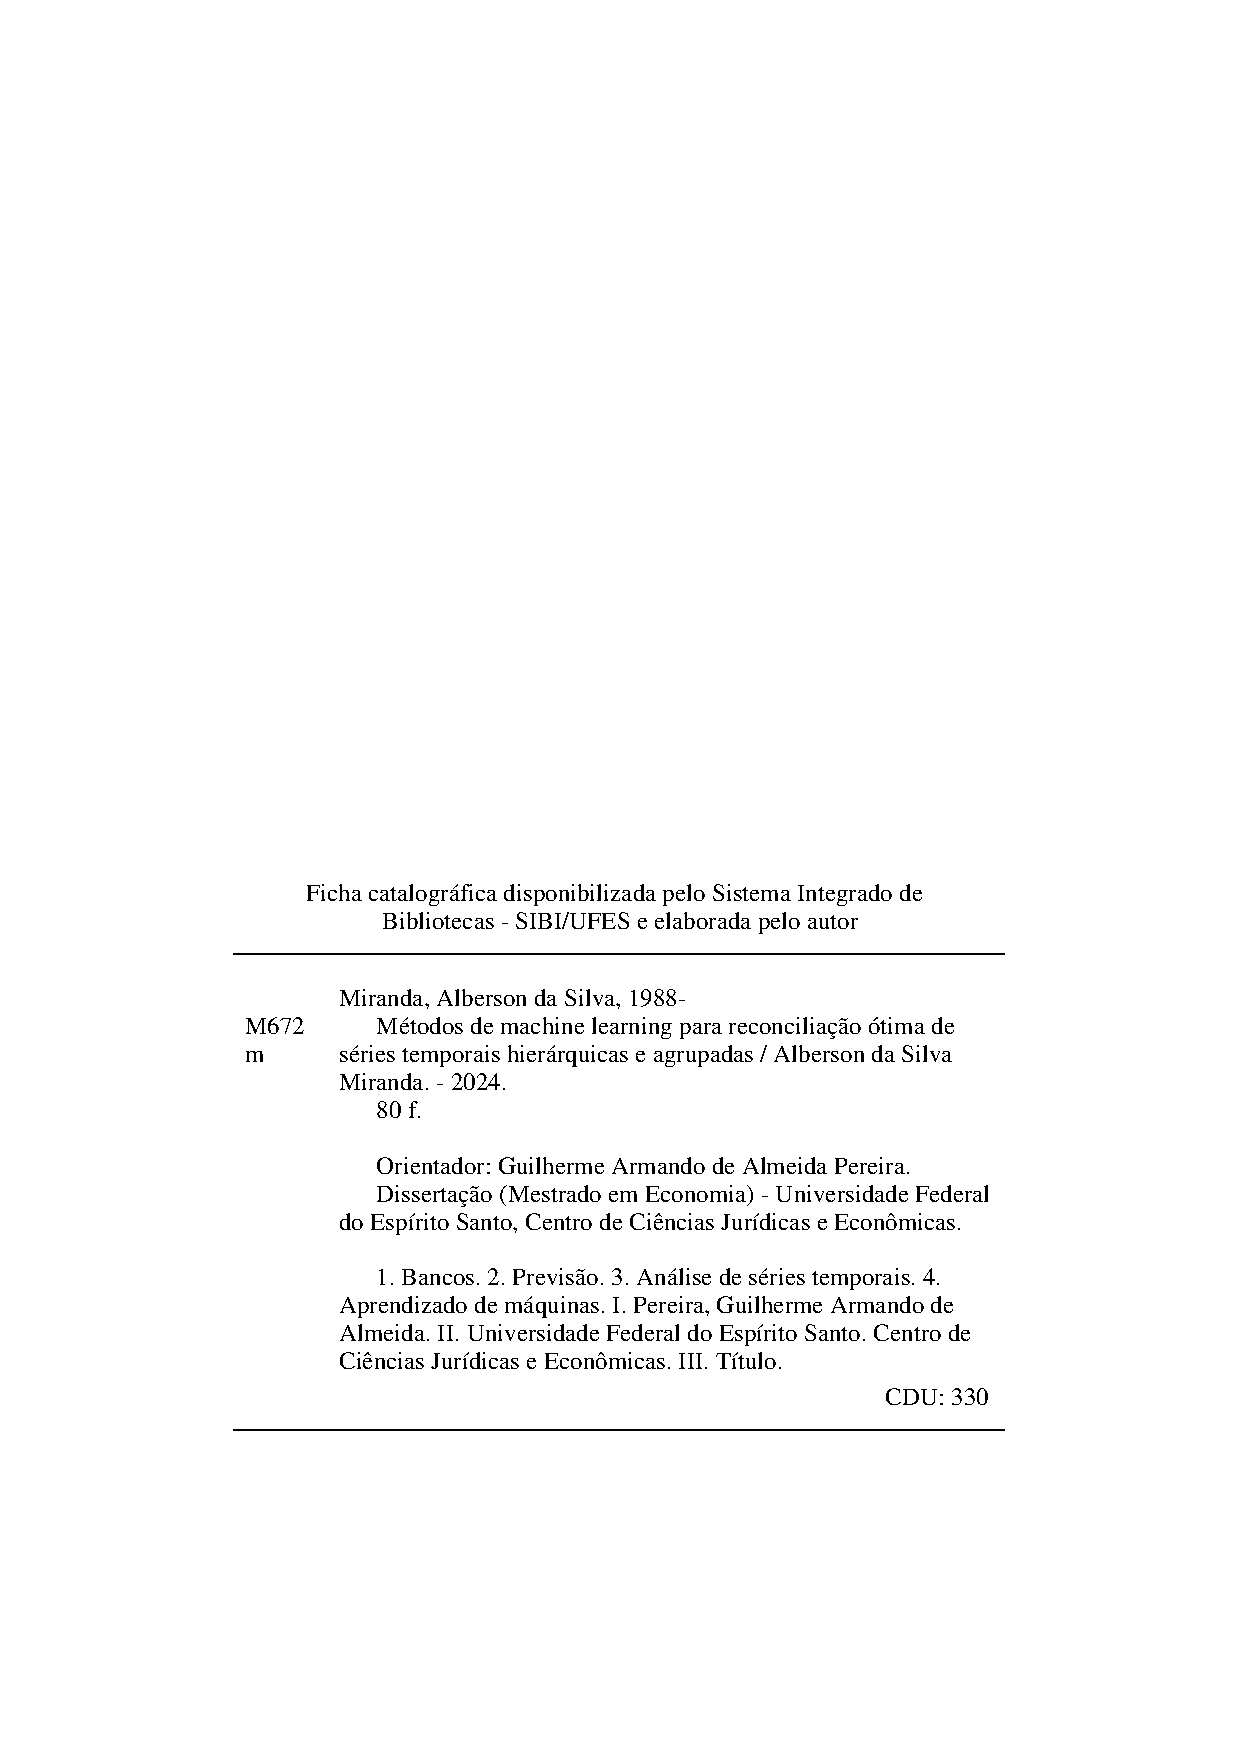
\includepdf{ficha_ufes.pdf}
%\end{fichacatalografica}


% substituir pela ficha em pdf fornecida pela UFES após defesa 
\begin{fichacatalografica}
	\sffamily
	\vspace*{\fill}					% Posição vertical
	\begin{center}					% Minipage Centralizado
	\fbox{\begin{minipage}[c][8cm]{15cm}		% Largura
	\small
	\imprimirautor
	
	\hspace{0.5cm} \imprimirtitulo  / \imprimirautor. --
	\imprimirlocal, \imprimirdata-
	
	\hspace{0.5cm} \thelastpage p. : il. (algumas color.) ; 30 cm.\\
	
	\hspace{0.5cm} \imprimirorientadorRotulo~\imprimirorientador\\
	
	\hspace{0.5cm}
	\parbox[t]{\textwidth}{\imprimirtipotrabalho~--~\imprimirinstituicao,
	\imprimirdata.}\\
	
	\hspace{0.5cm}
		1. Economia Bancária.
		2. Séries Temporais Hierárquicas.
		3. Reconciliação Ótima.
    4. Machine Learning.
		I. Pereira, Guilherme Armando de Almeida.
		II. Universidade Federal do Espírito Santo.
		III. Centro de Ciências Jurídicas e Econômicas.
		IV. Título 			
	\end{minipage}}
	\end{center}
\end{fichacatalografica}

% folha de aprovação 
%
%\begin{folhadeaprovacao}
%    \includepdf{folhadeaprovacao_final.pdf}
%\end{folhadeaprovacao}


% substituir pela folha assinada pela banca após defesa 
\begin{folhadeaprovacao}

  \begin{center}
    {\ABNTEXchapterfont\large\imprimirautor}

    \vspace*{\fill}\vspace*{\fill}
    \begin{center}
      \ABNTEXchapterfont\bfseries\Large\imprimirtitulo
    \end{center}
    \vspace*{\fill}
    
    \hspace{.45\textwidth}
    \begin{minipage}{.5\textwidth}
        \imprimirpreambulo
        \vspace*{1cm}
        Aprovada em 29 de fevereiro de 2024.\\[2cm]
        \textbf{COMISSÃO EXAMINADORA} \\
        \assinatura{\textbf{\imprimirorientador} \\ Universidade Federal do Espírito Santo \\ Orientador} 
        \assinatura{\textbf{Prof. Dr. Edson Zambon Monte} \\ Universidade Federal do Espírito Santo}
        \assinatura{\textbf{Prof. Dr. Fernando Luiz Cyrino Oliveira} \\ PUC-Rio}
        %\assinatura{\textbf{Professor} \\ Convidado 3}
        %\assinatura{\textbf{Professor} \\ Convidado 4}
    \end{minipage}%
   \end{center}
  
\end{folhadeaprovacao}

%% dedicatória 
%\begin{dedicatoria}
%   \vspace*{\fill}
%   \centering
%   \noindent
%   \textit{Exemplo de dedicatória,\\\lipsum[10].} \vspace*{\fill}
%\end{dedicatoria}

%% agradecimentos 
%\begin{agradecimentos}
%\lipsum[30]
%
%\lipsum[30]
%
%\end{agradecimentos}

% epígrafe 
%\begin{epigrafe}
%    \vspace*{\fill}
%	\begin{flushright}
%		\textit{``Modelo de epígrafe, \\
%		modelo de epígrafe.''}
%	\end{flushright}
%\end{epigrafe}

% resumo 

\setlength{\absparsep}{18pt}
\begin{resumo}
  O campo de pesquisa em métodos para previsões de séries temporais hierárquicas tem se mostrado fértil na última década, com seus avanços contribuindo para ganhos de acurácia na previsão de uma ampla gama de coleções de séries temporais. Recentemente, métodos de \textit{machine learning} (ML) têm sido incorporados à literatura de séries temporais hierárquicas, com trabalhos como os de \textcite{spiliotis_hierarchical_2021} e \textcite{makridakis_m5_2022} demonstrando resultados promissores. Este trabalho estende a exploração desses métodos na reconciliação ótima de séries temporais hierárquicas e agrupadas, investigando abordagens como \textit{random forest}, \textit{gradient boosting}, \textit{elastic net} e \textit{support vector machines}, e avaliando tanto sua performance preditiva quanto sua praticidade em termos de tempo de processamento. Além disso, o trabalho explora os efeitos de diferentes estratégias de obtenção do conjunto de treinamento para os modelos de ML, utilizando previsões para dentro da amostra obtidas via \textit{rolling origin forecasting}, valores ajustados de modelos reestimados (\textit{reduced fitted base}) e valores ajustados dos modelos de previsão base (\textit{fitted base}). Para avaliar a metodologia proposta, foram realizados três estudos de caso, sendo o primeiro relacionado a uma aplicação em economia bancária no Brasil, enquanto os demais envolvem bases de dados relacionadas ao setor de turismo doméstico australiano, amplamente utilizadas na literatura de séries temporais hierárquicas: 1. previsão de saldos de empréstimos e financiamentos do Banco do Estado do Espírito Santo; 2. previsão da quantidade trimestral de viagens; e 3. previsão da quantidade mensal de noites que os visitantes passam em viagens. Os resultados revelam que não há método ou estratégia que alcance consistentemente a melhor performance em todas as bases de dados ou níveis hierárquicos. Portanto, a escolha do método de reconciliação e da estratégia para obtenção do conjunto de treinamento depende não apenas da amostra, mas também do nível hierárquico de interesse do pesquisador. A combinação correta do método de ML e da estratégia pode resultar em até 91\% de ganho de performance em relação aos métodos analíticos de reconciliação ótima..

  \textbf{Palavras-chave}: Séries Temporais Hierárquicas. Reconciliação Ótima. \textit{Machine Learning}. Economia Bancária.
\end{resumo}

% abstract 
\begin{resumo}[Abstract]
  \begin{otherlanguage*}{english}
    
    In the past decade, the field of hierarchical time series forecasting has witnessed significant growth, marked by advancements that have enhanced accuracy of predicting a wide variety of time series. Recently, machine learning (ML) methods have been incorporated into the literature on hierarchical time series, with works such as those by \textcite{spiliotis_hierarchical_2021} and \textcite{makridakis_m5_2022} demonstrating promising results. This thesis builds upon these advancements, further exploring the potential of ML methods for optimal reconciliation of hierarchical and grouped time series by investigating approaches such as random forest, gradient boosting, elastic net and support vector machines. It assesses both their predictive performance and practical feasibility in terms of processing time. Moreover, the thesis investigates the impact of various training set acquisition strategies for ML models. These strategies include in-sample forecasts obtained through rolling origin forecasting, fitted values of reestimated models, and fitted values of base forecasts models. To evaluate the proposed methodology, three case studies were undertaken. The initial case study focuses on applying ML reconciliation in the context of Brazilian banking economics. Subsequent studies center on Australian domestic tourism datasets, which are frequently referenced in hierarchical time series literature. These include forecasting loan and financing balances for the State Bank of Espírito Santo (Brazil), quarterly overnight trips, and monthly visitor nights. The findings reveal that no single method or strategy consistently outperforms others across all datasets or hierarchical levels. Thus, the choice of reconciliation method and training set strategy hinges not only on the sample but also on the researcher's specific hierarchical level of interest. Nonetheless, the appropriate combination of ML method and strategy can yield up to a 91\% improvement in accuracy compared to the best-performing analytical reconciliation method.
    \vspace{\onelineskip}
 
    \noindent 
    \textbf{Keywords}: Hierarchical Time-Series. Optimal Reconciliation. Machine Learning. Economics of Banking.
  \end{otherlanguage*}
\end{resumo}

% lista de ilustrações 
\pdfbookmark[0]{\listfigurename}{lof}
\listoffigures*
\cleardoublepage

% lista de quadros 
%\pdfbookmark[0]{\listofquadrosname}{loq}
%\listofquadros*
%\cleardoublepage

% lista de tabelas 
\pdfbookmark[0]{\listtablename}{lot}
\listoftables*
\cleardoublepage

% lista de abreviaturas 
\begin{siglas}
  \item[ETS] \textit{Exponentional Smoothing}
  \item[Favar] \textit{Factor Augmented Vector Autoregression}
  \item[Lasso] \textit{Least Absolute Shrinkage and Selection Operator}
  \item[MCRL] Modelo Clássico de Regressão Linear
  \item[MASE] \textit{Mean Absolute Scaled Error}
  \item[MinT] \textit{Minimum Trace}
  \item[MQGF] Mínimos Quadrados Generalizados Factíveis
  \item[MQO] Mínimos Quadrados Ordinários
  \item[MQP] Mínimos Quadrados Ponderados
  \item[PIB] Produto Interno Bruto
  \item[RMSSE] \textit{Root Mean Squared Scaled Error}
  \item[SFN] Sistema Financeiro Nacional
  \item[SVR] \textit{Support Vector Regression}
  \item[XGBoost] \textit{Extreme Gradient Boosting}
\end{siglas}

% lista de símbolos 
\begin{simbolos}
  \item[$ t $] Tempo dentro da amostra
  \item[$ T $] Último tempo dentro da amostra
  \item[$ h $] Horizonte de previsão, tempo fora da amostra
  \item[$ \Omega $] Conjunto de dados dentro da amostra
  \item[$ y $] Série temporal dentro da amostra
  \item[$ \hat{y} $] Série temporal estimada
  \item[$ \tilde{y} $] Série temporal reconciliada
  \item[$ n $] Número de séries na hierarquia
  \item[$ m $] Número de séries no menor nível da hierarquia
  \item[$ k $] Número de níveis na hierarquia
  \item[$ \mathbfit{S} $] Matriz de soma
  \item[$ \mathbfit{G} $] Matriz de reconciliação
  \item[$\{...\}$] Conjunto
  \item[$|\{...\}|$] Cardinalidade de um conjunto
\end{simbolos}

% sumário 
\pdfbookmark[0]{\contentsname}{toc}
\tableofcontents*
\cleardoublepage

% elementos textuais 
\textual
\pagestyle{simple}